\documentclass[Main.tex]{subfiles}
\begin{document}
\section{Experimenten en resultaten}
Voor het verklaren van de experimenten zijn er een aantal zaken die vermeld moeten worden. De meeste experimenten zijn gebaseerd op de resultaten van de voorgaande experimenten. Daarom worden de experimenten in een bepaalde volgorde uitgevoerd. Er worden verschillende beoordelingswijzen gebruikt bij het onderzoeken van de experimenten. Enerzijds testen de experimenten op oplossingsgraad\footnotemark[\ref{note:oplossingsgraad}] en anderzijds op de tijd die het algoritme nodig heeft. 
\par Indien er geen rekening gehouden wordt met de resultaten van vorige experimenten, dan zijn sommige van de latere experimenten enorm tijdrovend. Deze laatste tonen ook niets aan wat niet aangetoond kan worden met de resultaten uit de voorgaande experimenten. \par Alle experimenten zijn uitgevoerd op een \textit{2.26 GHz Intel Core 2 Duo} processor en zijn uitgevoerd met 500 iteraties. Deze zijn gedaan op een bewerkingsboom met diepte vijf, tenzij anders vermeld. Een bewerkingsboom van diepte vijf betekent dat vergelijkingingen zoals $A^{B}+C \div D \ast E$ met vijf waarden gevonden kunnen worden maar $A^{B}+C \div D \ast E \ast A$ met zes waarden niet. Bij elk van deze iteraties worden er twee voorbeelden gegeven waaraan de vergelijking moet voldoen. De experimenten volgen de subhypothesen in sectie \ref{ssec:subhypothesen}.  

\subsection{Pruning in bewerkingsboom} \label{ssec:pruning}
In dit experiment wordt er onderzocht of de zoekruimte gecre\"eerd door de bewerkingsboom niet verkleind kan worden. Zoals aangehaald in sectie \ref{ssec:Prunen} kan prunen in de bewerkingsboom de zoekruimte enorm verkleinen. Vooral omdat een absoluut redundante knoop ervoor zorgt dat al zijn kinderen nutteloos zijn. Wanneer deze dus weggehaald wordt vallen alle kinderen ook weg. In dit experiment zal bekeken worden hoeveel knopen er nu juist kunnen gepruned worden. Op experimentele wijze wordt nu onderzocht hoeveel knopen overbodig zijn in de bewerkingsboom. Hiervoor wordt er een vergelijking gemaakt tussen het aantal knopen van de originele boom en het aantal knopen in deze nieuwe boom.
\par Zoals weergegeven in Figuur \ref{fig:pruningInBewerkingsboom} blijven er 65\% van de knopen over. Dit heeft als gevolg dat bij het uitwerken van de bewerkingsboom 35\% minder vergelijkingen zullen moeten doorlopen worden. Het prunen op zich vraagt natuurlijk ook tijd. Daarom is de optie om de boom op voorhand te berekenen bekeken. Uit korte experimenten bleek echter al snel dat het voordeel klein is op lage diepte. De besparing ligt ongeveer rond de $100$ ms. Omdat het prunen van de uitwerking moeilijker is in deze geprunede bewerkingsboom is er vervolgens geopteerd om de boom niet op voorhand te berekenen.

\begin{figure}[!htb]
\centering
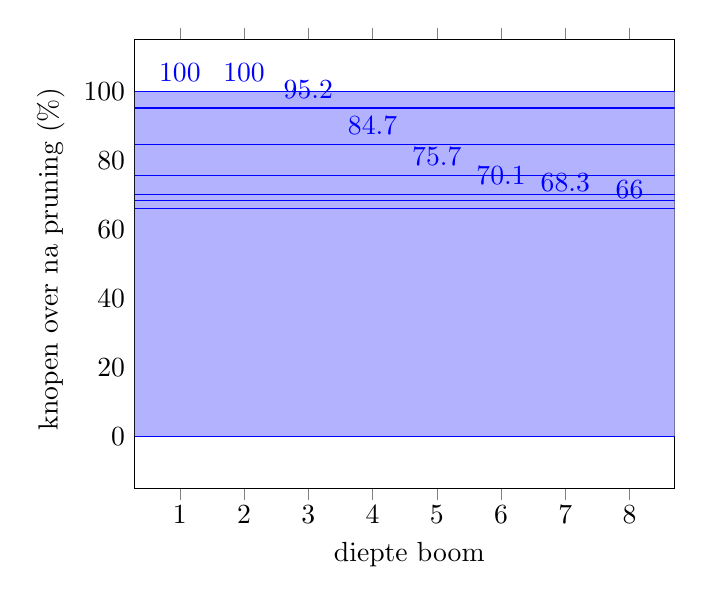
\begin{tikzpicture}
  \begin{axis}[
    ybar,
    ymax = 100,
	ymin = 0,
    enlarge x limits=0.1,
    enlarge y limits=0.15,
    ylabel={\ knopen over na pruning (\%)},
    xlabel={\ diepte boom},
    xtick=data,
    nodes near coords, 
	nodes near coords align={vertical},
    x tick label style={rotate=0,anchor=mid,yshift=-1.5ex},
    bar width=20,
    ]
    \addplot coordinates {(1, 100) (2, 100) (3,95.2) (4,84.7) (5,75.7) (6,70.1) (7,68.3) (8,66.0)};
  \end{axis}
\end{tikzpicture}
\caption{Resultaat pruning in bewerkingsboom.} \label{fig:pruningInBewerkingsboom}
\end{figure}

\subsection{Constanten} \label{ssec:constanten}
Volgens subhypothesen 1 en 2 uit sectie \ref{ssec:subhypothesen} heeft het toevoegen van constanten een positieve invloed op de oplossingsgraad. Hieruit kan een optimale set van constanten gevonden worden.
De volgende stap is het bepalen wat de invloed van het toevoegen van constanten heeft op de snelheid en de oplossingsgraad van het algoritme. In dit experiment worden er drie verschillende sets van constanten gebruikt. Deze zijn: $(1,2,3), (1,2,3,4,5)$ en $(1,2,3,5,7)$. De redenering achter deze sets van getallen is dat de toevoeging van slechts \'e\'en of twee constanten een te beperkte invloed zou hebben. Het verschil tussen de invloeden van een set waarin drie of vier constanten zitten is ook beperkt, daarom is er gekozen voor een set van vijf constanten. De laatste set is een verzameling van 1 en de priemgetallen met een waarde kleiner dan tien. De reden hiervoor is dat elk getal groter dan twee uitgedrukt kan worden door een combinatie van priemgetallen.
\par Deze experimenten zijn uitgevoerd op een boom waar reeds de redundante knopen (zie experiment \ref{ssec:pruning}) zijn uitgehaald. Om goed te kunnen vergelijken wordt zowel in Figuur \ref{fig:gewichtenTijd} als in Figuur \ref{fig:gewichtenOplossingsgraad} ook het resultaat zonder constanten getoond. Wanneer we Figuur \ref{fig:gewichtenTijd} en Figuur \ref{fig:gewichtenOplossingsgraad} naast elkaar leggen, kan er besloten worden dat het gebruik van $(1,2,3,5,7)$ het beste resultaat oplevert. De grafieken spreken voor zich, behalve wanneer het gebruik van de constanten $(1, 2, 3, 4, 5)$  wordt vergeleken met het gebruik de constanten $(1, 2, 3, 5, 7)$ . De oplossingsgraad van deze tweede set van constanten ligt hoger, omdat aan de hand deze constanten gemakkelijker andere constanten gevormd kunnen worden. De doorlooptijd bij het gebruik van de constanten $(1, 2, 3, 4, 5)$ ligt lager dan deze bij $(1,2,3,5,7)$ door de gebruikte manier van prunen. Het is namelijk niet toegelaten dat het combineren van constanten reeds bestaande constanten genereert. Bij de set $(1, 2, 3, 4, 5)$ komt dit nu eenmaal vaker voor en dus worden er meer knopen gepruned waardoor er minder vergelijkingen moeten worden doorlopen.

%TODO mooiere benaming assen
\begin{figure}[!htb]
\centering
\begin{tikzpicture}
  \begin{axis}[
    ybar,
    enlarge x limits=0.2,
    enlarge y limits=0.15,
    ylabel={\ tijd (ms)},
    xlabel={\ gebruikte set constanten},
    symbolic x coords={$leeg$,${1, 2, 3}$,${1, 2, 3, 5, 7}$,${1, 2, 3, 4, 5}$,},
    xtick=data,
    nodes near coords, 
	nodes near coords align={vertical},
    x tick label style={rotate=0,anchor=mid,yshift=-1.5ex},
    bar width=30,
    ]
    \addplot coordinates {($leeg$, 625.6) (${1, 2, 3}$, 4029.5) (${1, 2, 3, 5, 7}$, 15269.3) (${1, 2, 3, 4, 5}$, 15934.7)};
  \end{axis}
\end{tikzpicture}
\caption{Vergelijking van de nodige tijd met het gebruik van constanten.} \label{fig:gewichtenTijd}
\end{figure}



\par Als algemene conclusie van dit experiment kan gesteld worden dat het gebruik van constanten weldegelijk een positieve invloed heeft. De zoektijd moet dan wel beperkt kunnen worden. De keuze van de set $(1, 2, 3, 5, 7)$ biedt de beste verhouding tussen een verhoging van de oplossingsgraad en de vertraging. In de verdere experimenten zullen deze constanten dan ook gebruikt worden. Het is belangrijk om op te merken dat de mogelijkheid bestaat dat de gebruiker een voorbeeld geeft die exact deze waarden bevat. Bovendien is er niet ge\"experimenteerd met constanten die waarden groter dan tien bevatten omdat er niet verwacht wordt dat de gebruiker zulke vergelijkingen zoekt.


%TODO mooiere benaming assen
\begin{figure}[!htb]
\centering
\begin{tikzpicture}
  \begin{axis}[
    ybar,
    ymax = 100,
	ymin = 0,
    enlarge x limits=0.2,
    enlarge y limits=0.15,
    ylabel={\ oplossingsgraad (\%)},
    xlabel={\ gebruikte set constanten},
    symbolic x coords={$leeg$,${1, 2, 3}$,${1, 2, 3, 5, 7}$,${1, 2, 3, 4, 5}$,},
    xtick=data,
    nodes near coords, 
	nodes near coords align={vertical},
    x tick label style={rotate=0,anchor=mid,yshift=-1.5ex},
    bar width=30,
    ]
    \addplot coordinates {($leeg$, 54.2) (${1, 2, 3}$, 78.4) (${1, 2, 3, 5, 7}$, 94.3) (${1, 2, 3, 4, 5}$, 85.7)};
  \end{axis}
\end{tikzpicture}
\caption{Vergelijking van de oplossingsgraad bij het gebruik van constanten.} \label{fig:gewichtenOplossingsgraad}
\end{figure}

\subsection{Brute force vs Optimaliseren}
In de laatste sectie zal het 'brute force algorithm' vergeleken worden met het geoptimaliseerde algoritme, wat overeenkomt met de laatste subhypothese uit sectie \ref{ssec:subhypothesen}. In Figuur \ref{fig:brutevsopttijd} wordt de onderlinge tijd vergeleken. Er wordt waargenomen dat het geoptimaliseerde algoritme weldegelijk sneller de boom doorloopt. Naarmate er dieper wordt gezocht neemt het tijdsverschil toe, maar beide algoritmes blijven exponentieel toenemen in tijd. De oplossingsgraad van beide zijn ongeveer gelijk. Het geoptimaliseerde algoritme vindt in bepaalde situaties betere oplossingen. Hiermee worden vergelijkingen bedoeld die meer in het verwachtingspatroon van de gebruiker liggen. De gebruiker heeft liever een vergelijking waarin weinig constanten worden gebruikt, maar wel alle gegeven waarden. Desondanks de betere oplossingen en snellere uitvoeringstijd zijn de resultaten eerder negatief. Daarom is er gezocht naar een eventuele heuristiek om de zoekboom sneller te doorlopen. Er werd geen heuristiek gevonden, omdat de productieregels van de contextvrije grammatica toelaten dat de resulaten van ouder naar kind enorm verschillen.


\begin{figure}[!htb]
\centering
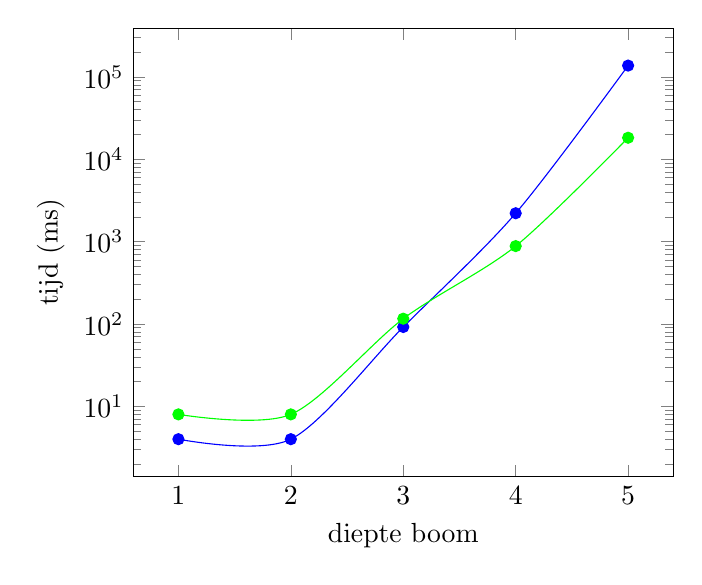
\begin{tikzpicture}
\begin{axis}[
	ymode=log,
	xlabel=diepte boom,
	ylabel=tijd (ms),
	xtick=data,]
\addplot[smooth,mark=*,blue] coordinates {
	(1,   4)
	(2,   4)
	(3,   92)
	(4,   2209)
	(5,   136920)
};
\addplot[smooth,mark=*,green] coordinates {
	(1,   8)
	(2,   8)
	(3,   116)
	(4,   882)
	(5,   18223)
};
\end{axis}
\end{tikzpicture}
\caption{Vergelijking van de tijd die het 'brute force algorithm' nodig heeft en die het geoptimaliseerde algoritme nodig heeft om 5 niveaus diep te berekenen.} \label{fig:brutevsopttijd}
\end{figure}

\end{document}